\documentclass{article}

\usepackage{amsmath}
\usepackage{amsfonts}
\usepackage{listings}
\usepackage{a4wide}
\usepackage{hyperref}
\usepackage{color}
\usepackage{chngcntr}
\usepackage{titling}
\usepackage{pdfpages}
\usepackage{wrapfig}
\usepackage{floatrow}
\usepackage{subcaption}


\numberwithin{equation}{section}

\hypersetup{
    colorlinks,
    citecolor=black,
    filecolor=black,
    linkcolor=black,
    urlcolor=black
}

\definecolor{mygreen}{rgb}{0,0.6,0}
\definecolor{mygray}{rgb}{0.5,0.5,0.5}
\definecolor{mymauve}{rgb}{0.58,0,0.82}

\lstset{ %
    backgroundcolor=\color{white},   % choose the background color
    basicstyle=\footnotesize,        % size of fonts used for the code
    breaklines=true,                 % automatic line breaking only at whitespace
    captionpos=b,                    % sets the caption-position to bottom
    commentstyle=\color{mygreen},    % comment style
    escapeinside={\%*}{*)},          % if you want to add LaTeX within your code
    keywordstyle=\color{blue},       % keyword style
    stringstyle=\color{mymauve},     % string literal style
}

\title{24MAC175 Group 1 Coursework Report}
\author{Matthew Lakin, James Death, Nathan Moore, Saad Tahir}
\date{November - December 2024}
\pretitle{\begin{center}\Huge}
\posttitle{\end{center}\vskip 0.5em}

\begin{document}
\maketitle
\newpage
\tableofcontents
\newpage

\section{Algorithm Explanation}
The question we recieved  isn't able to be solved using the Simplex Method as it is. The Simplex Method is used to solve linear programming problems exclusively in the canonical form. So the first step is to sanitise the question and put it in the correct form.
\subsection{Converting to Canonical Form}
The question we were asked to solve was as follows: \\ \\
Minimise $z = 7x_1 + 11x_3 - 10x_4 - x_5 + 26x_6$,\\Subject to constraints:
\begin{align}
    x_1 - x_2 + x_3 + x_5 + x_6 &= 76  \label{lpp1:constraint1} \\
    x_2 - x_3 + x_4 + 3x_6 &\leq 18 \label{lpp1:constraint2} \\
    x_1 + x_2 - 3x_3 + x_4 + x_5 &\leq 12 \label{lpp1:constraint3} \\
    x_1 + x_2 + x_6 &\geq 50 \label{lpp1:constraint4}
\end{align}
with all variables non-negative: $x_1, x_2, x_3, x_4, x_5, x_6 \geq 0$. \\ 

The first step in solving this is to put it into canonical form. Canonical form is where the question is in the form:
\begin{align}
    \text{Minimise }z &= \underline{c}^T \cdot \underline{x} \\
    A\underline{x} &= \underline{b} \\
    \underline{x} &\geq 0
\end{align}
For this, we add slack and surplus variables to (\ref{lpp1:constraint1}), (\ref{lpp1:constraint2}), and (\ref{lpp1:constraint3}) to remove the inequality in favour of an equality: \\ \\
Minimise $z = 7x_1 + 11x_3 - 10x_4 - x_5 + 26x_6$, subject to
\begin{align}
    x_1 - x_2 + x_3 + x_5 + x_6 &= 76 \label{lpp2:constraint1} \\
    x_2 - x_3 + x_4 + 3x_6 + S_1 &= 18 \label{lpp2:constraint2} \\
    x_1 + x_2 - 3x_3 + x_4 + x_5 + S_2 &= 12 \label{lpp2:constraint3} \\
    x_1 + x_2 + x_6 - S_3&= 50 \label{lpp2:constraint4}
\end{align}
with all variables non-negative: $x_1, x_2, x_3, x_4, x_5, x_6, S_1, S_2, S_3\geq 0$.\\ \\
However (\ref{lpp2:constraint4}) violates the non-negativity constraint, so to fix that we need to introduce artificial variables to the LPP. In order to make a basic feasible solution we need to add artificial variables to both (\ref{lpp2:constraint1}) and (\ref{lpp2:constraint4}). We will also amend the objective function with a large M value. This will be used in calculations so the artificial variables tend to 0 as iterations progress. So now the problem becomes: \\ \\
Minimise $z = 7x_1 + 11x_3 - 10x_4 - x_5 + 26x_6 + M(R_1 + R_2)$, subject to
\begin{align}
    x_1 - x_2 + x_3 + x_5 + x_6 + R_1&= 76 \\
    x_2 - x_3 + x_4 + 3x_6 + S_1 &= 18 \\
    x_1 + x_2 - 3x_3 + x_4 + x_5 + S_2 &= 12 \\
    x_1 + x_2 + x_6 - S_3 +R_2 &= 50
\end{align}
with all variables non-negative: $x_1, x_2, x_3, x_4, x_5, x_6, S_1, S_2, S_3, R_1, R_2\geq 0$.\\
\newpage
The LPP is now in canonical form and is ready for simplex.

\subsection{Revised Simplex Algorithm}
The Revised Simplex Algorithm is a variant of the Simplex Algorithm. Instead of using a tableau, it uses a matrix to store values.\\ \\
The question consists of m constraints and n variables. We use slack, surplus and artificial variables to create a basic feasible solution. Iterating through all possible basic solutions is not a viable method since the amount of possible basic solutions is $\binom{n}{m}$ which grows factorially.\\
Our implementation of the Revised Simplex Algorithm follows these steps:
\begin{enumerate}
    \item Partition the matrix into the basis and non-basis variables, B and N respectively.
    \item Compute a basic solution.
    \item Using the dual matrix, compute the reduced costs.
    \item If all reduced costs are non-negative, the solution is optimal and the algorithm terminates.
    \item If not, select the most negative reduced cost as the entering variable.
    \item A direction vector $d_B$ is calculated by multplying the B matrix with the vector of the entering variable.
    \item We find the ratios between the right-hand side and the direction vector. The smallest ratio is the leaving variable.
    \item We update the basis and repeat the process until the solution is optimal.
\end{enumerate}
\newpage
\section{Worked Example}
On paper, we solved a slightly simpler version of the question we were given. We did this to verify the Simplex Method. The solution is below: \\ \\
\includegraphics[width=\textwidth]{Media/Cut 1.png}
\includegraphics[width=\textwidth]{Media/Cut 2.png}
\includegraphics[width=\textwidth]{Media/Cut 3.png}
\newpage
\section{Implementation}
For this project, we used Python for access to the NumPy module and MatPlotLib for graphing. The code was written in a modular fashion, with each function performing a specific task.
\subsection{Representation of the Problem}
Before doing any simplex calculations on the question, we had to parse the question into a form that python could understand. For our representation, we used 5 data structures:
\begin{itemize}
    \item Nature: This is a binary value that represents whether the problem is a maximisation or minimisation problem. If the problem is a maximisation problem, the value is -1, otherwise it is 1.
    \item A: This is a matrix that represents the coefficients of the constraints. Each row represents a constraint, and each column represents a variable.
    \item b: This is a vector that represents the right-hand side of the constraints. Each row represents a constraint.
    \item c: This is a vector that represents the coefficients of the objective function. Each column represents a variable.
    \item Signs: This is a vector that represents the signs of the constraints. Each row represents a constraint. The value -1 represents a less than or equal to constraint, 0 represents an equal to constraint, and 1 represents a greater than or equal to constraint.
\end{itemize}
As we have code to convert the LPP (Linear Programming Problem) to canonical form, we can accept any LPP in any form.
\subsection{Main Method}
The main method is the entry point for the program. It is where the question is inputted and the functions are called. When using this project, this is the only method that needs to be interacted with.
\subsection{Converting to Canonical Form}
The function convertToCanonicalForm in file bfs.py is used to convert the LPP to canonical form. The function takes the LPP in our parsing style as input and returns the LPP in canonical form. It also introduces artificial variables to the LPP to make a basic feasible solution along with amending the objective function with a large M value if required.\\
The function requires a valid LPP to work. We added a check to see if the LPP is valid before running the function.\\
It takes each constraint and does 1 of 3 things:
\begin{itemize}
    \item If the constraint is an equality constraint, it adds an artificial variable to the constraint.
    \item If the constraint is a less than or equal to constraint, it adds a slack variable to the constraint.
    \item If the constraint is a greater than or equal to constraint, it adds a surplus and an artificial variable to the constraint.
\end{itemize}

\subsection{Simplex Method}
The function revisedSimplexMethod in file simplex.py is used to solve the LPP in canonical form.\\ 
This uses the exact same algorithm as described in the Algorithm Explanation section. It uses the optimality test to determine if the current solution is optimal. If it is not, it gives the entering variable and uses the feasibility test to find the leaving variable. It then updates the bases and repeats until the solution is optimal.\\
It also checks for infeasibility and unboundedness. If the LPP is infeasible, it returns "Solution is Infeasible". If the LPP is unbounded, it returns "Unbounded solution".

\subsection{Parsing the LPP}
The function renderLPP in file render.py is used to render the LPP. It supports LPP, both canonical and non-canonical form. The function takes the LPP in our parsing style as input and returns a string representation of the LPP.

\subsection{Graphing}
The function graph in file variableGraphing.py is used to graph the variables. To change which constraint is being varied, you need to change the variable "bVaryNum". Then the function will make a graph of all feasible solutions which exist in the interval [1, 200].\\
If the interval of feasible solutions is smaller than 200, the interval will be reduced to the size of the feasible interval.

\subsection{Using the Code}
To use the code to answer the provided question, you must verify that variables in main.py are set correctly. The variables are as follows:
\begin{lstlisting}[language=Python, basicstyle=\scriptsize, frame=single]
    nature = 1
    c = nature * np.array([7, 0, 11, -10, -1, 26])
    A = np.array([[1, -1, 1, 0, 1, 1], [0, 1, -1, 1, 0, 3], [1, 1, -3, 1, 1, 0], [1, 1, 0, 0, 0, 1]])
    b = np.array([76, 18, 12, 50])
    signs = np.array([0, -1, -1, 1])
\end{lstlisting}
Once you run main.py, you should see the multiple iterations with each entering and leaving variable and at the end the optimal solution. If the solution is infeasible or unbounded, it will print that instead:
\begin{lstlisting}
    ---------------------------------------------------------------------------
    Optimal Value:  200
    Optimal Solution:  [49.2  0.8 27.6 44.8  0.   0.   0.   0.   0.   0.   0. ]
    Status:  Optimal solution found
    ---------------------------------------------------------------------------
\end{lstlisting}

\newpage
\section{Special Cases}
\subsection{Infeasible Solutions}
We performed an analysis which investigates whether the solution remains feasible when the constraints of the LPP are altered by varying the value of b.  This was completed using MATLAB's LPP solver. The package systematically adjusted the b values of each constraint independently and gave the number 1 when the solution was feasible and 0 when unfeasible. We concluded when adjusting constraint 1, the solution became infeasible at an extreme b value. This occurred when the b value was decreased by 100 from 76 to -24. We then verified the solution was infeasible using the python "SciPy" simplex package and it produced the following:
\begin{lstlisting}
    The problem is infeasible. (HiGHS Status 8: model_status is Infeasible; primal_status is At lower/fixed bound)
\end{lstlisting}
From this analysis we now have an example of a definitive infeasible problem to test against the implemented algorithm. At first when testing this problem we had to alter the input slightly to accept the negative b value. We did this by multiplying the whole constraint 1 by -1 and inputting it into the code as the following parameters:
\begin{lstlisting}[language=Python, basicstyle=\scriptsize, frame=single]
    nature = 1                                             
    c = nature * np.array([7, 0, 11, -10, -1, 26])
    A = np.array([[-1, 1, -1, 0, -1, -1], [0, 1, -1, 1, 0, 3], [1, 1, -3, 1, 1, 0], [1, 1, 0, 0, 0, 1]])
    b = np.array([24, 18, 12, 50])
    signs = np.array([0, -1, -1, 1])
\end{lstlisting}
This should produce an infeasible solution as the b value is 24 in order to maintain a positive however to compensate the first constraint in "A" has swapped signs in all values in order to simulate a b value of -24. After an initial test it did produce an optimal value as well as corresponding solution of variables. 
\begin{lstlisting}
    ---------------------------------------------------------------------------
    Optimal Value:  6682
    Optimal Solution:  [ 0. 50. 32.  0.  0.  0.  6.  0. 58.  0.  0.]
    Status:  Optimal solution found
    ---------------------------------------------------------------------------
\end{lstlisting}
Not only was the optimal value unusually large compared to previous data but the optimal solution had a 'non-zero' value as an artificial variable. Since the simplex algorithm was not able to filter out all artificial variables to 0 the problem is indeed infeasible. To counteract this problem so that the algorithm can account for other potential infeasible solutions, we adapted the code to check the artificial variables in the optimal solution. It would conclude a status  'Optimal solution found' only if all artificial variables equated to 0. After rerunning the same problem it produced the following:
\begin{lstlisting}
    ---------------------------------------------------------------------------
    Solution is Infeasible.
    ---------------------------------------------------------------------------
\end{lstlisting}
\newpage
\subsection{Unbounded Solutions}
Additionally we wanted to test the algorithm against an unbounded example. We found an unbounded example online that reads:
\begin{align}
    \text{Maximise }z &= 6x + 8y \\
    \text{Subject to }x - y &\geq 0, \\
    -x + 3y &\leq 3, \\
    x, y &\geq 0
\end{align}
In order to confirm it was an unbounded LPP we ran the input against the 'SciPy' package as before and it confirmed the LPP had an unbounded solution.
\begin{lstlisting}[language=Python, basicstyle=\scriptsize, frame=single]
    nature = -1                                            
    c = nature * np.array([6, 8])
    A = np.array([[1, -1], [-1, 3], [1, 1]])
    b = np.array([0, 3, 0])
    signs = np.array([1, -1, 1]) 
\end{lstlisting}
Our implemented algorithm checks if the solution is unbounded each iteration thus if it concludes the solution is unbounded it will change the status to 'Unbounded solution' .
Against this example it worked as intended and printed the following, after 4 iterations, rather than an optimal solution:
\begin{lstlisting}
    ---------------------------------------------------------------------------
    Solution is Unbounded.
    ---------------------------------------------------------------------------
\end{lstlisting}
\newpage
\section{Verification}
For verification, we admitted the question: \\
Minimise $z = 7x_1 + 11x_3 - 10x_4 - x_5 + 26x_6$, subject to
\begin{align}
    x_1 - x_2 + x_3 + x_5 + x_6 &= 76 \label{ver1:constraint1} \\
    x_2 - x_3 + x_4 + 3x_6 &\leq 18 \label{ver1:constraint2} \\
    x_1 + x_2 - 3x_3 + x_4 + x_5 &\leq 12 \label{ver1:constraint3} \\
    x_1 + x_2 + x_6 &\geq 50 \label{ver1:constraint4}
\end{align}
with all variables non-negative: $x_1, x_2, x_3, x_4, x_5, x_6 \geq 0$. \\
We then used the Python package SciPy to solve the question. The representation of the question in SciPy is as follows:
\begin{lstlisting}[language=Python, basicstyle=\scriptsize, frame=single]
    import numpy as np
    from scipy.optimize import linprog

    c = np.array([7, 0, 11, -10,-1,26])
    Aup = np.array([[0, 1, -1, 1, 0, 3],
                    [1, 1, -3, 1, 1, 0],
                    [-1, -1, 0, 0, 0, -1]])
    bup = np.array([18, 12, -50])
    Aeq = np.array([[1, -1, 1, 0, 1, 1]])
    beq = np.array([76])
\end{lstlisting}
Since SciPy's method doesn't support the greater than or equal to constraints, we had to alter (\ref{ver1:constraint4}) by multiplying both sides of the equation by -1 and flipping the inequality. 
\begin{equation}
    -x_1 - x_2 - x_6 \leq -50
\end{equation}
We then used the SciPy method linprog to solve the question. The results were as follows:
\begin{lstlisting}[language=Python, basicstyle=\scriptsize, frame=single]
    res = linprog(c,Aup,bup,Aeq,beq)
    print(res)
\end{lstlisting}
\begin{lstlisting}[language=Python, basicstyle=\scriptsize]
    message: Optimization terminated successfully. (HiGHS Status 7: Optimal)
    success: True
     status: 0
        fun: 200.0
          x: [ 4.920e+01  8.000e-01  2.760e+01  4.480e+01  0.000e+00
               0.000e+00]
        nit: 5
      lower:  residual: [ 4.920e+01  8.000e-01  2.760e+01  4.480e+01
                          0.000e+00  0.000e+00]
             marginals: [ 0.000e+00  0.000e+00  0.000e+00  0.000e+00
                          1.000e+00  4.500e+01]
      upper:  residual: [       inf        inf        inf        inf
                                inf        inf]
             marginals: [ 0.000e+00  0.000e+00  0.000e+00  0.000e+00
                          0.000e+00  0.000e+00]
      eqlin:  residual: [ 0.000e+00]
             marginals: [-1.000e+00]
    ineqlin:  residual: [ 0.000e+00  0.000e+00  0.000e+00]
             marginals: [-9.000e+00 -1.000e+00 -9.000e+00]
    mip_node_count: 0
    mip_dual_bound: 0.0
    mip_gap: 0.0
\end{lstlisting}
The solution of the question corresponds with the "fun" value in the dictionary output. The value of the objective function is 200.0, which matches the value we found using the Revised Simplex Method. It also shows it took 5 iterations in the "nit" value which also aligns itself with our calculations. This verifies that our implementation is correct for this question.
\newpage
\begin{figure}
    \centering
    \begin{subfigure}{.5\textwidth}
      \centering
      \includegraphics[width=\linewidth]{Media/Graphs/Constraint2MatLab.jpg}
    \end{subfigure}%
    \begin{subfigure}{.5\textwidth}
      \centering
      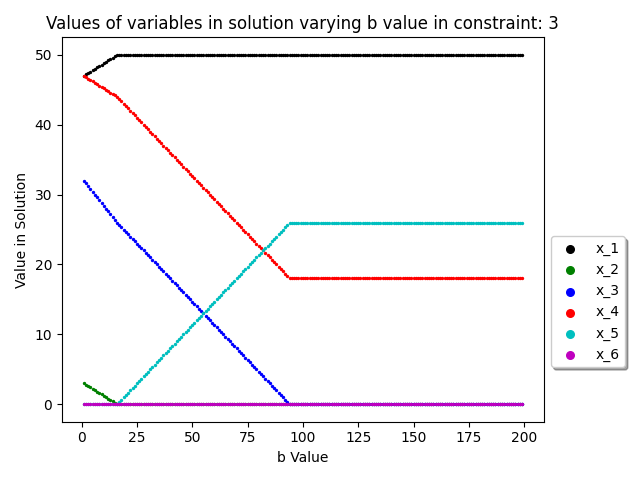
\includegraphics[width=\linewidth]{Media/Graphs/valuesVaryb3.png}
    \end{subfigure}
    \caption{Left: MATLAB Sensitivity Analysis, Right: Python Sensitivity Analysis}
\end{figure}
We displayed the variables in the solution changing b in constraint 3 calculated using a MATLAB package, and our implemented algorithm in Python. \\
We did this to ensure that all solutions match up with the MATLAB package. \\
Notable similarities can be observed between the graphs:
\begin{itemize}
    \item $x_1$ and $x_2$ have an intersection at b = 1
    \item At b = 16, $x_2$ leaves the basis and $x_5$ enters the basis
    \item The trajectories of $x_3$ and $x_5$ are on course to intersect in the MATLAB graph as shown in the Python graph.
\end{itemize}
\newpage
\section{Sensitivity Analysis}
\subsection{Behaviour of the Objective Function}
\begin{wrapfigure}{r}{0.6\textwidth}
    \centering
    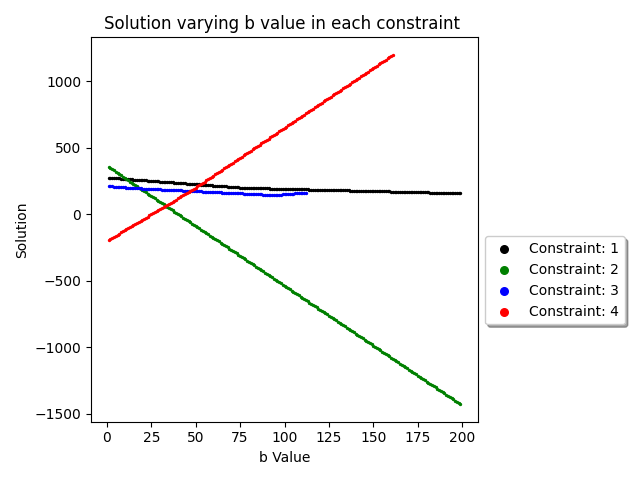
\includegraphics[width=0.6\textwidth]{Media/Graphs/solutionsVaryb.png}
\end{wrapfigure}
From this graph a clear idea of the strengths of the constraints can be shown. Firstly, constraints 2 and 4 show the greatest strength, this is shown through the smallest of adjustments to their value, massively impacts the solution. This can't be said for constraints 1 and 3, as from the graph it shows that when altered, the solution doesn't change much and stays fairy level. Furthermore, the graph highlights the infeasibility of certain constraints and when this takes place. For constraint 3, this is for values over 112 where the line is cut off, meaning the solution has become infeasible. Similarly for constraint 4, over 161 is where the line cuts off and the solution is infeasible. In order to produce a smaller optimal solution, increasing the b value of constraint 2 will minimise the solution the greatest. Constraint 4 is the opposite, where increasing the b will directly hinder the minimisation process by increasing the optimal solution the most. \\ \\
If the constraints were treated as a weight, then we can calculate their worth via the gradient of their respective lines in the graph:
\begin{itemize}
    \item Constraint 1: at b=1, Solution = 276 and at b = 200, Solution = 157.33,    Gradient = -0.596
    \item Constraint 2: at b=1, Solution = 357.33 and at b = 200, Solution = -1438, Gradient= -9.022
    \item Constraint 3: at b=1, Solution = 211 and at b = 200, Solution = 144, Gradient = -0.337
    \item Constraint 4: at b=1, Solution = -193.33333 and at b = 200, Solution = 1626, Gradient = 9.142
\end{itemize}
\subsection{Constraint 1}
\begin{wrapfigure}{r}{0.6\textwidth}
    \centering
    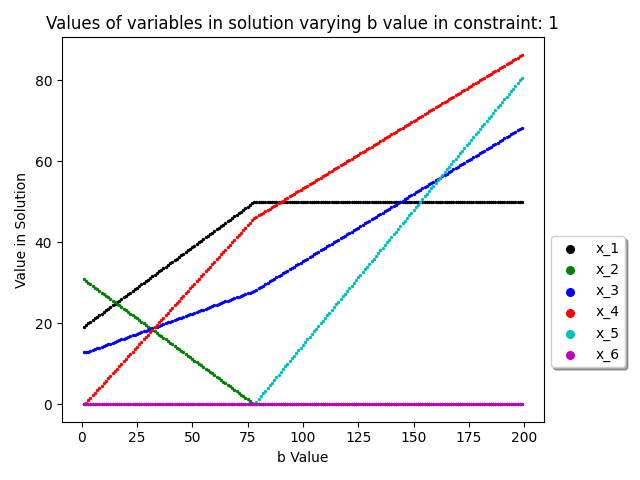
\includegraphics[width=0.6\textwidth]{Media/Graphs/valuesVaryb1.png}
\end{wrapfigure}
It can be seen that both variables $x_3$ and $x_4$ steadily increase at near the same rate, as the b value is increased. Furthermore, the same with all the constraints, there is a shift in the basis variables of $x_2$ and $x_5$ which can be highlighted. This is where when one variable is contributing, the other one is not involved and is zero. It can be seen, $x_1$ variable after the b value of 78 stay consistent from then on. 
\newpage
\subsection{Constraint 2}
\begin{wrapfigure}{r}{0.6\textwidth}
    \centering
    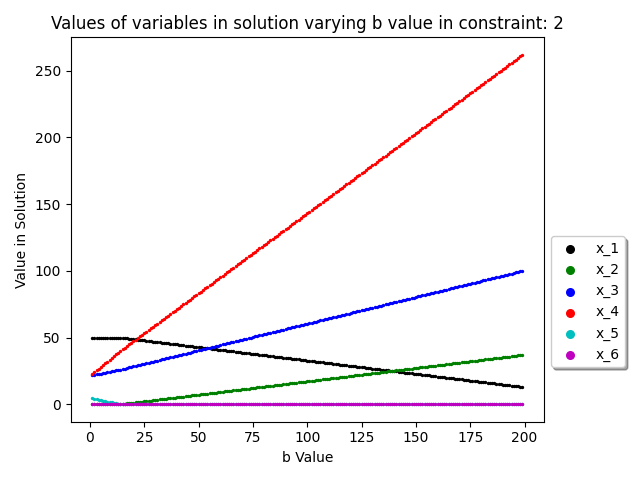
\includegraphics[width=0.6\textwidth]{Media/Graphs/valuesVaryb2.png}
\end{wrapfigure}
We notice variable $x_4$ consistently increases as the b value is increased, this shows its importance and when relaxing the constraint resources are reallocated to $x_4$, for an optimal solution. The non-basic variable $x_5$ becomes active for the extremely low b values, where $x_1$ is seen to steadily decrease, crossing over with multiple other variables.  Both variables $x_2$ and $x_3$ follow the same trajectory upwards as the b value is increased. 
\subsection{Constraint 3}
\begin{wrapfigure}{r}{0.6\textwidth}
    \centering
    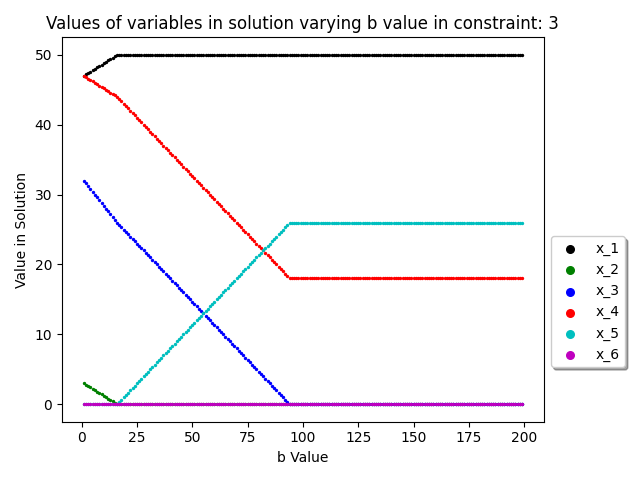
\includegraphics[width=0.6\textwidth]{Media/Graphs/valuesVaryb3.png}
\end{wrapfigure}
Again, $x_1$ staying the same value from around a b value of 17 to 93 but drops rapidly at the extremely high b values. This takes places at the same time variable $x_2$ becomes active again and increases fast. The non-basic variable $x_6$ remains inactive, as it does in all constraints. Variable $x_5$ is observed to be very strong in this constraint and is very clearly important for the optimality. 
\subsection{Constraint 4}
\begin{wrapfigure}{r}{0.6\textwidth}
    \centering
    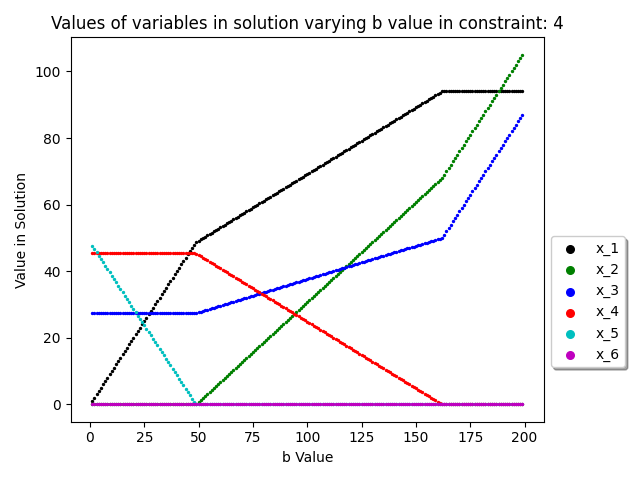
\includegraphics[width=0.6\textwidth]{Media/Graphs/valuesVaryb4.png}
\end{wrapfigure}
In this constraint the crossover of variables $x_1$ and $x_4$ can be seen clearly, where when the b value is increased, $x_1$ increases whilst $x_4$ decreases. This relationship suggests $x_1$ and $x_4$ are competing variables in this constraint and so respond inversely to changes to the b value. The same $x_2$ and $x_5$ relationship is shown, with $x_5$ leaving, as $x_2$ enters. The variable $x_3$ is seen to steadily increase as the b value increases, when passed b = 44. 
\newpage
\section{Conclusion}
Through this project, we have produced a functioning implementation of the Revised Simplex Method in Python.
We have verified the implementation using SciPy's linprog function and MATLAB's LPP solver.\\
We have analysed the behaviour of the objective function when varying the constraints of the LPP and explained what it means in the context of the question.\\ \\
After much testing, we have calculated the result of: \\
Minimise $z = 7x_1 + 11x_3 - 10x_4 - x_5 + 26x_6$, subject to
\begin{align}
    x_1 - x_2 + x_3 + x_5 + x_6 &= 76 \\
    x_2 - x_3 + x_4 + 3x_6 &\leq 18 \\
    x_1 + x_2 - 3x_3 + x_4 + x_5 &\leq 12 \\
    x_1 + x_2 + x_6 &\geq 50
\end{align}
with all variables non-negative: $x_1, x_2, x_3, x_4, x_5, x_6 \geq 0$. \\ 
is equal to 200 with the optimal solution of:
\begin{align}
    \underline{x} = \begin{bmatrix}
        49.2 \\
        0.8 \\
        27.6 \\
        44.8 \\
        0 \\
        0
    \end{bmatrix}
\end{align}
We parsed the question into this form: \\
\begin{lstlisting}[language=Python, basicstyle=\scriptsize, frame=single]
    nature = 1
    c = nature * np.array([7, 0, 11, -10, -1, 26])
    A = np.array([[1, -1, 1, 0, 1, 1], [0, 1, -1, 1, 0, 3], [1, 1, -3, 1, 1, 0], [1, 1, 0, 0, 0, 1]])
    b = np.array([76, 18, 12, 50])
    signs = np.array([0, -1, -1, 1])
\end{lstlisting}
and produced the output of:
\begin{lstlisting}
    ---------------------------------------------------------------------------
    Optimal Value:  200
    Optimal Solution:  [49.2  0.8 27.6 44.8  0.   0.   0.   0.   0.   0.   0. ]
    Status:  Optimal solution found
    ---------------------------------------------------------------------------
\end{lstlisting}
This code can be used to solve other LPP's. It will also check for special cases such as infeasibility and unboundedness. \\


\end{document}